\part{Context, Requirements and State-of-the-Art Review}
%\setcounter{chapter}{0}

%%  une page de citation (pas indispensable)
%\vspace{12cm}

~\vspace{1cm}
\begin{flushright}
{\it Every person I work with knows something better than me.\\
My job is to listen long enough to find it and use it.}\\
Jack Nichols
\end{flushright}
\vspace{2cm}

The European population is getting older due to a conjunction of two factors. First, the decrease of births reduced the part of youth in the population. The second factor is the soon arrival of post-war "baby-boom" people to the age of retirement. Both of these factors imply a radical change in the age pyramid, and in the socio-economical environment of European countries. A consequence of this ageing of the population is an emergence of needs and requirements to face this global evolution.
\par Over the past few years, home automation technologies have been tending to democratize. More and more technical solutions are proposed to automate shutters, garage doors or lightning in houses. These facilities improved the quality of life of the European population. Now they sound like an interesting tool that could help and offer support to elderly people in their home.\\

As an introduction, chapter~\ref{ch:introduction} presents the Ambient Assisted Living and Home Automation domains, in order to extract some general requirements and outline the contribution of this thesis.\\
After this introduction, a state-of-the-art review in AAL projects, Home Automation, and software engineering approaches is carried out in chapter~\ref{ch:survey}. 
Chapter \ref{ch:summary} ends this first part with a summary of the state of the art, and announces the contribution of this thesis.


\chapter{Introduction}
\label{ch:introduction}


Home Automation and the Ambient Assisted Living(AAL) domains have been of major influence on this work. Home Automation technologies offered a plethora of technical solutions with various constraints, while AAL brought substantial real life material in terms of requirements, needs, or use cases.\\
This introduction chapter presents these domains in sections~\ref{sec:context.aal} and~\ref{sec:context.homeautomation}. This presentation enables section~\ref{ch:requirements} to list some general requirements identified in these domains. Section~\ref{sec:scope} defines the scope of this work before section~\ref{sec:introContrib} outlines the contribution of this thesis.


\section{Ambient Assisted Living}
\label{sec:context.aal}

\begin{wrapfigure}{r}{60mm}
	\vspace{-0.5cm}
  \centering
  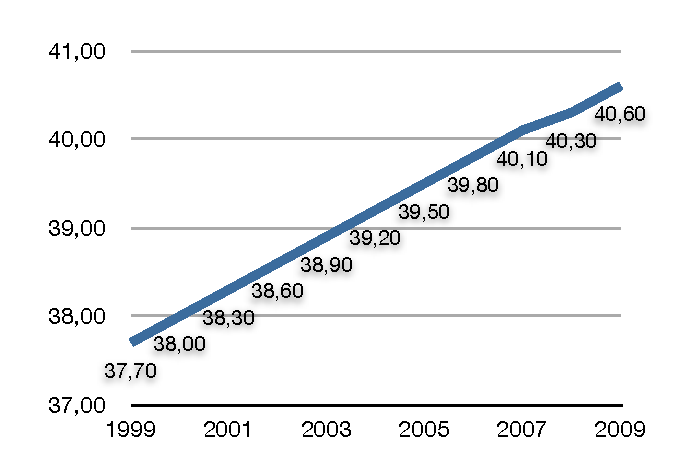
\includegraphics[width=60mm]{part1/pics/medianAgeEUPop.pdf}
  \caption{Median Age of EU Population - Source Eurostat}
    \label{fig:medAge}
	\vspace{-0.5cm}
\end{wrapfigure}

\subsection{The origins}

According to Eurostat~\footnote{http://epp.eurostat.ec.europa.eu/portal/page/portal/eurostat/home}, the median age of European Union (27 countries) population has been growing regularly. From a median age of 37.7 years in 1999, it increased to 40.6 years in 2009 as shown on figure~\ref{fig:medAge}. It is a fact; the European population is getting older each year. This ageing of the population is the result of the combination of several factors, among which are the ageing of baby-boomers, and the decrease of birth rates.\\

The {\bf "Baby Boom"}\\
During the Second World War the birth rate stagnated, resulting in a similar number of births from 1939 to 1945. This stagnation is visible in figure~\ref{fig:agePyramidEU272009}, at the level of people aged between 64 and 70. The "Baby Boom" describes the rapid and strong increase in the number of births that occurred after the Second World War, thus between 1945 and 1968. Actually, 4.9 million people were born in 1944 in the EU, 7.6 million were born in 1968 (+35.8\%). People born during the "Baby Boom" are now (in 2011) 43 to 68 years old, and will soon retire.\\

{\bf Decrease in birth rates}\\
As can be noticed in figure~\ref{fig:agePyramidEU272009}, a decrease in birth rates began at the end of the sixties. From 7.664 million persons born in 1968, the number of births fell to 5.061 million in 2002 (-33.4\%). In \cite{Bosch:1998}, Xavier Bosch explains that this phenomenon is due to a multitude of factors such as an increase in the use of contraception, the raise of the number of single people, or the increase in the percentage of women in the workforce.\\

\begin{wrapfigure}{r}{60mm}
	%\vspace{-0.8cm}
  \centering
  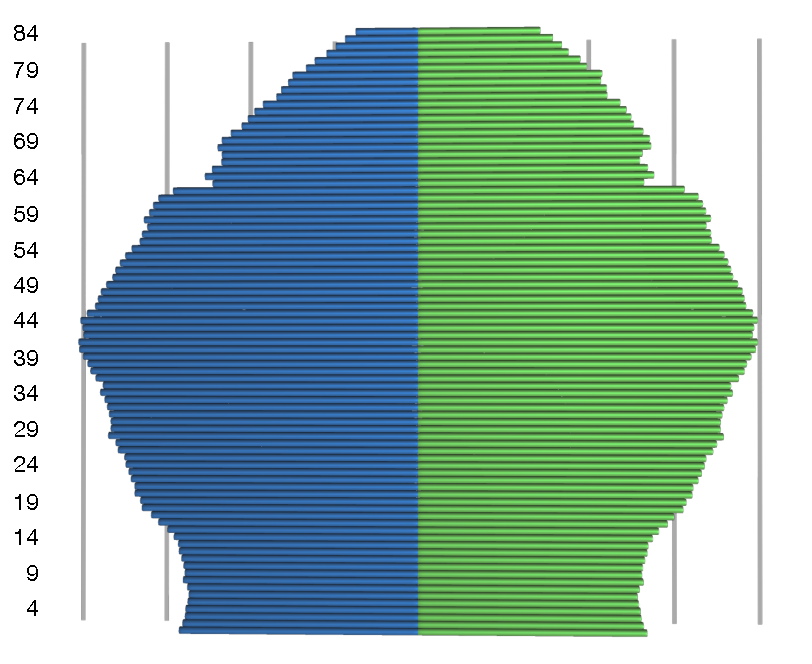
\includegraphics[width=60mm]{part1/pics/AgePyramidEU272009.pdf}
  \vspace{-0.8cm}
  \caption{Age Pyramid EU (27) in 2009. - Blue: M, Green: F - Source Eurostat}
  \label{fig:agePyramidEU272009}
	\vspace{-0.5cm}  
\end{wrapfigure}

Europe will soon have to face the increase in the retired portion of the population, and a simultaneous decrease in young people entering working life. By 2050, the number of people over 65 in the EU will have increased by 70\%, and the number of people over 80 will have grown by 170 \%.\\

In order to be ready on time, governments must address the economic and social implications of an ageing population. They must prepare for increasing demands on healthcare, as a rapidly ageing society heralds growing populations with chronic diseases, disabilities, and increasing health needs.\\

\subsection{The concept}
\label{subsec:aalConcepts}

The Ambient Assisted Living Joint Programme~\cite{jointAALProgram} defines the concept of \gls{aal} through 6 dimensions.\\
{\bf Autonomy} By increasing the autonomy, the self-confidence and the mobility of elderly people, \gls{aal} tends to extend the length of time people can live in their preferred environment. \\
{\bf Activities} Maintaining physical or intellectual exercise helps elderly people to remain in good health, and prevents a decrease in capacities.\\
{\bf Assisting} individuals at risk, by promoting a better and healthier lifestyle.\\
{\bf Securing} support and maintaining the network around the individual, including family, friends and social activities, to enhance security and prevent social isolation.\\
{\bf Supporting} carers, families and care organizations in their everyday activities.\\
{\bf Streamlining} the use of resources dedicated to elderly people, by increasing their efficiency and productivity.\\

There are many solutions to address these dimensions. Automation of some tasks can enforce autonomy, and the use of mechanical aids can improve mobility. Social workers and health professionals can propose activities, support and assistance. Unfortunately, healthcare associations or companies have difficulty in hiring people for these jobs. Indeed, qualified people are not numerous enough, and financial constraints are strong in this domain.\\
~\vspace{0.5cm}

A solution, in assisting both helped people and helpers, could be to use Home Automation technologies in conjunction with ICTs and human interventions. Section \ref{sec:context.homeautomation} presents this domain.



\section{Home Automation}
\label{sec:context.homeautomation}

%\begin{wrapfigure}{r}{40mm}
%	\vspace{-0.5cm}
%  \centering
%  
\includegraphics[width=40mm]{part1/pics/Jetsons.jpeg}
%  \caption{The Jetsons}
%	\vspace{-0.5cm}  
%\end{wrapfigure}

In 1962, William Hanna and Joseph Barbera created the Jetsons cartoon family. In this carton, George and Jane were living in the \textit{Skypad Apartments} in \textit{Orbit City} with their children Judy and Elroy. Their housekeeping robot, Rose, handled all chores not done by the numerous automated appliances triggered with some push-buttons. Apart from the fact that it is just a fiction cartoon, it describes well the idea of smart homes or home automation. Let us get into a bit more detail about home automation, and see why it is still not applied in everyone's home.


\subsection{Application domains}
Home automation has for too long been perceived as it was presented in the Jetsons: a set of costly, useless, funny pieces of technology.\\
Obviously, personal home theaters, multi-room media systems, smart colored lighting controllers will always exist and make a good showcase of what is possible. Besides, the use of more utility-oriented home automation is soaring. Home or building automation technologies, among others, ease the management of lighting control, shutter control, heating, ventilation, air conditioning, energy management, metering, monitoring, alarm/intrusion systems, household appliances, audio/video and lots more. However, people are not ready to pay for the automation of tasks they can execute by themselves.\\
Widely used in industry buildings and plants, the automation of the lighting or heating systems has brought substantial savings of energy and money. This industrial experience makes it possible to imagine the benefits of installing such systems in homes. The minimization of power consumption with a maximization of welfare is acceptable, even dreamed of by everybody.
By extension, alarm systems, automatic garage doors and shutters can also be managed this way, rendering a global and coherent service to inhabitants. 

\subsection{Technologies}

The devices encountered in home automation originate from different business domains. M. Nagy says in~\cite{Terziyan:2009} that "A major problem is inherent heterogeneity [...] with respect to nature of components, standards, data formats, protocols, [...]". Indeed, it can be a problem from many aspects, but it is also a set of tools waiting to be connected.\\

{\bf Communication Media}\\
Four main communication media can be differentiated in home automation technologies: the {\it Bus}, the {\it Radio}, the {\it \gls{plc}} and {\it Infrared}.
Devices use these communication media to communicate with each other, and offer a technical functionality.
The choice of a medium is linked to the constraints to be addressed. For instance, a Bus link is highly reliable, but requires the wiring of the entire house. On the other hand, Radio communications do not need any additional wiring, but are less reliable and batteries have to be changed regularly.\\

{\bf Plethora of protocols}\\
Historically, there is no specific home automation brand or manufacturer. It all comes from different trades such as electricity or \gls{hvac} control. According to the specific needs of their domains, each home automation manufacturer has developed a specific communication protocol for its devices to operate with each other. They also use several communication media to carry the communications. A consequence of that is the huge number of devices, protocols and media available on the home automation market, illustrated in section~\ref{subsection:homeAutomationDetails}. 
Technical solutions proposed by the Home Automation domain are so numerous, that there may be a solution for each need, in almost each domain. Nevertheless, due to this great diversification, no common management tool exists so far, resulting in expensive mono-manufacturer closed solutions, or no solution at all.\\
Even if home automation technologies have existed for many years, no real standard has been released. Imposing a global standard, as was the case for the IP protocol for example, seems to be the best way to address such an issue. Naturally, each domain has created its communication protocol adapted to each business concern. Thus, finding a common protocol, used and understood by all devices from all domains, appears to be a very difficult task. And even if one finally emerges, developers will still have to deal with legacy devices using proprietary protocols.\\
Moreover, the old way manufacturers think adds to the complexity of the problem. They still think that a closed world (I mean non-public protocol specifications) is a world that can be controlled. Indeed, it is true, but it is also a world that fewer and fewer people want to enter, because they are afraid of the captivity imposed by such solutions. Captive systems are often well tested, because of the  restricted number of available devices, but there is also a risk for these components of being removed from the market one day. In these conditions, people could not replace these components with compatible others, and are thus really concerned with the sustainability of the adopted solution.\\



\section{Identification of requirements}
\label{ch:requirements}

The domain of Home Automation requires a new breed of technology to easily manage installations and answer specific needs. The lack of such a tool, able to operate any home automation technology and create solutions for specific needs of elderly people, makes the adoption and use of these technologies marginal. This absence of a tool may be due to the complexity and number of requirements inherent to home automation systems. This section aims to identify a set of required properties for a software tool to be adopted by manufacturers, installers and users.\\

The requirements presented in this section had been identified in \cite{Nain09a}. This section completes the list and elaborates on them.\\


%\subsection{Required properties}

{\bf Interoperability}\\
Interoperability is described as the ability for systems to operate with each other. Even if 'system' is quite a generic word and encompasses lots of things, the idea behind interoperability is simple. Given two or more systems, how can one ensure that each of them is operable with another one? For instance, if I have a light management system and another one for shutters, how can I guarantee that systems will be able to communicate in order to be of use for the user?\\
A closed environment, in which all devices come from the same manufacturer, avoids the problem. A communication interface, common to all components, also deals with the issue.
Interoperability becomes a complex problem when the environment is open and when several technical concerns have to be handled in a single place (lighting and heating management for instance).\\
In the context of \gls{aal}, each solution will be uniquely deployed, because each patient, each helped person has specific needs due to his environment or illness. Indeed, specialists in this domain will select different technical artifacts or services, according to each person's needs. Those solutions will have to cooperate with each other in a single system, to perfectly meet the user's needs, whoever their manufacturer or whatever their communication protocol may be.\\


{\bf Openness}\\
Openness means making all offered functionalities available for third party applications, or different uses other than the one initially imagined. 
In closed systems, customers are limited to the functionalities and evolutions proposed by the solution's manufacturer. If the system deployed was built specifically for a customer, any evolution is very costly. Keeping the system open to external contributions may reduce the number of demands for costly system modifications or add-ons. In any case, it is also an open door for new unforeseen appliances adding smart behavior to a reliable set of functionalities.\\
This is a clear challenge in computer sciences, and in general when considering communications and interactions between objects or systems. 
The definition of a home-made interface fulfilling the requirements is easier than fitting into a good practice or a standard that does "almost what we want but not completely".\\
Openness is a strong requirement in home automation systems, as it has been in computers. Today, a computer manufacturer would not create a specific connection port, compatible with no other computer, unless he wants to create a new captive market.\\

{\bf Adaptation}\\
In a perfect world, devices never fail, services are always available and the Internet is always available. As demonstrated every day, the world we are living in is not perfect. Software systems, or systems dealing with objects or services linked to everyday life actions, have to take their execution environments into consideration. They should be able to dynamically adapt to changes around them while they are running, in order to maintain a given level of services or functionality as long as possible. Obviously, these adaptations should not require any reboot of the system, because a reboot could make all in-house functionalities unavailable. Lastly, an adaptation is not intended to add or remove any system functionality permanently. Otherwise, it is an evolution.\\
Execution policies or system reactions must be easily modifiable, in order to take into account any change in the user's requirements. For instance, depending on the level of dependency of an elderly person, the system may completely, partially or not at all automate the management of certain household functions such as heating or shutter management. This type of change in system behavior has to be made simple and operable by any authorized person, even with no specific skill in this domain.\\
Most of all, these changes during runtime must not affect the execution of basic security functions (such as emergency call handling), neither in their behavior, nor in their execution during adaptation.\\
Adaptations do not only concern technical elements, but also the user himself. All users are different. While some may be interested in new technologies, others are completely agnostic. When some are able to remember and learn how the system behaves, others may experience some memory loss. Where some have vision disorders, others experience hearing limitations. Software systems should be able to take into account these disabilities and adapt to their evolutions and to users' requirements.\\

{\bf Evolution}\\
Evolution in the context of home automation and/or assisted living is a key requirement. Needs or uses are changing, protocols and technologies also. Some functionalities may finally be required, whereas others can become useless and need to be uninstalled. Security or communication protocols can be improved and deployed in new versions that have to be taken into account without needing to re-implement the entire system.\\
Moreover, systems deployed in a house or a building, in charge of its management and the comfort of its inhabitants, have to be designed to serve during the entire lifetime of the building (even if hardware changes may be required). Therefore, they must be ready to accommodate future and unforeseen evolutions such as the installation of new services/functionalities for example.\\

{\bf Variability Management}\\
No house or building is like any other. This is because of structural or ground specificities, because of a particular user's need or just because no one would like to have exactly the same house as his neighbor. Thus, each installation will have specific devices deployed, using specific versions of protocols, and providing several functionalities. The development, by hand, of a specific control system for each installation is completely out of the question. It would be too costly and error prone. A global management tool should exist to deal with the inherent variability of such systems.\\
People responsible for designing a solution for an installation query should have some tools at their disposal to help them in choosing devices to install, or to assist them in selecting devices from all the catalogs of all manufacturers.\\

{\bf Remote Control}\\
More and more, people want to remotely access their belongings. This is also true for their homes. They would like to be able to remotely check the lights status, run a bath or switch on the alarm system that they forgot.\\
In the context of building management facilities, specialized companies have different solutions to check the state of a building system. They either have remote access to all systems, or they check locally by hand. Obviously, the local solution is longer viable in the context of our society. Systems deployed to control buildings or homes should have remote access possibilities (under access control and agreement) to allow for remote diagnosis, corrections, or evolution actions from a control center.\\

{\bf Distribution}\\
Today's systems work more and more with or on different execution platforms, and communicate more with each other. This is particularly true for home automation. For redundancy reasons and service level insurance a building and even a house can be equipped with multiple, independent, but connected controllers. These controllers can share the different functions to balance the loads on platforms, or offer a connection to a specific, locally-connected device. When a running platform fails, other platforms aware of its job can stand in temporarily, until the original controller is back in operation. Also, devices are becoming smarter and may make decisions by themselves. As a consequence, decisions and control could be distributed to several smart pieces of equipment.\\

{\bf Safety \& Security}\\
As presented in the context of this work, safety and security are very important requirements for home automation systems. Indeed, they themselves have to be safe and secured to be able to play their role in difficult situations and improve the security and safety of people and goods.
A minimum service level has to be guaranteed, for inhabitants not to remain stuck in the house in the case of an emergency. Moreover, the access policies of the system have to be sufficient to avoid unauthorized access, and simple enough not to become a constraint for authorized carers.\\
Several tools such as simulators, tests, or model checking, can be used to check and improve the reliability and the safety of such systems.\\

{\bf Acceptability \& Accessibility}\\
In the domain of home automation, deployed solutions, whatever their nature, have to take into consideration interactions with all inhabitants. Whether they are children, teenagers, young workers, parents, retired or old people, all of them must be able to interact with the system. 
Checks have to be performed on all solutions proposed, to ensure all users can control, or obtain information from the system and keep control.\\

New requirements for software are emerging from the accessibility of home automation technologies. The evolution of the software during the building's lifetime, its adaptation to cope with changes in its execution environment and the huge variability of technologies and protocols to be guaranteed to inter-operate, are triggering new challenges for software engineering.

\section{Scope of this work}
\label{sec:scope}
The list of requirements presented in the previous section could be completed. A particular situation can bring many other issues for software engineering.\\
This thesis focuses only on a subpart of these requirements and aims to propose a solution to conjunctively address interoperability, adaptation, openness, evolution, variability management and, partially, safety and security issues. The first goal of this thesis was to end up with a working solution able to cope with this sub-list of requirements. Other ones will be addressed in future works. As for safety and security issues, the work realized in this thesis partially addresses the problem, since questions about privacy and information security concerns have been decided as out of scope. The focus was more about ensuring consistency of assemblies and a fail-safe system.

\newpage
\section{Contribution of this thesis}
\label{sec:introContrib}

Software can no longer be built on a once-off basis. Customizable, reliable and personalized solutions have to be deployed in the short terms to meet changes in users' needs or in the environment at any time. Moreover, the specificities of each installation make it very hard to create a unique piece of software able to cope with all technologies, concerns (such as energy consumption) or unpredictable evolutions.\\

In the electronics domain, the number of components and their always-possible connectivity have offered technicians and engineers the means to create various solutions. Even many years after their assembly, electronic devices can still be repaired or completed with new features. The proposal made in this thesis is to take advantage of the electronic way of doing to improve the flexibility of software systems while keeping a high level of safety and security.\\
To this end, the contribution of this thesis can be described from three aspects:
\par - A constraint-relaxed component model that leverages the software flexibility, by offering ways to connect any component to any other. This aspect addresses interoperability issues and evolution requirements
\par - Modeling tools to create, modify and simulate component assemblies, check their consistency and validity before their (re-)deployment at runtime. Safety and security, as much as variability management are requirements covered by this aspect of the contribution.
\par - An execution environment built over a service-oriented runtime, to support the proposed component model and cope with adaptation and evolution requirements at runtime.\\


\chapter{State-of-the-Art Review}
\label{ch:survey}

The review proposed in this chapter is made if three sections.\\
Section~\ref{sec:background} starts with a description of the Ambient Assisted Living domain from which social requirements have emerged, and it presents some projects on this topic. It then introduces some home automation technologies, their use and goals in several projects. The overview of these two domains makes it possible to sense more precisely the needs for a new breed of software for these domains.\\
Section~\ref{sec:generalPurposeApproaches} then presents several general purpose software approaches and tools that have been considered for the resolution of the problem targeted. Each of them is evaluated against the requirements identified in the introduction. However, general purpose approaches seem not to be specialized enough to meet the requirements of the \gls{aal} and home automation domains.\\
For this reason, section~\ref{sec:domainSpecificApproaches} evaluates some selected domain-specific approaches with respect to the same requirements as for general purpose ones.\\
Finally, the review made in this chapter is summarized in chapter~\ref{ch:summary} which uses this basis to specify the contribution of this thesis.


\section{Background on AAL and Home Automation}
\label{sec:background}

Ambient Assisted Living is a hot topic in Europe. Several projects have been led to address different aspects and try to cover the needs inherent to a home-keeping situation. This section introduces some of them.

\subsection{Projects in AAL}

The \glsreset{aal}\gls{aal} Joint Programme~\footnote{http://www.aal-europe.eu} is a collaborative association of twenty European Union Member States, plus three Associated States. They group together the AAL Association, whose main objective is to enhance the quality of life of elderly people, through the use of \gls{ict}. Their main activity is to found R\&D projects in the \gls{aal} domain and to publish annual calls for project proposals.\\
The total budget planned for the \gls{aal} Joint Programme is €700 million, half of which is to be funded by public resources (AAL Partners plus the European Commission) and the other half by private participating organizations. According to the 13\up{th} article of the EC decisions 743/2008/EC~\cite{743/2008/EC}, funding from the European Commission is taken from the budget allocated to the \gls{ict} theme of 'Cooperation' under the FP7 Specific Programme of the same name. Thus, the \gls{aal}-JP is set to last from 2008 to 2013, to correspond to the FP7 dates.\\


The {\bf ASK-IT} project~\footnote{http://www.ask-it.org/ (march 2011)} ran from 2004 to 2008, and aimed at providing {\it Ambient Intelligence} to support and promote the mobility of impaired people~\cite{Wiethoff:2007}. It laid to the development of a software framework, and a set of tools for mobility. Among other things, a {\it Domestic Module} has been created to support the provision of seamless home environment management, to the mobility-impaired traveler on the move.\\

In a slightly similar approach, the {\bf SOPRANO} project~\footnote{http://www.soprano-ip.org/ (march 2011)} intends to design an \gls{ict} system to foster the comfort and safety of elderly people in their everyday life. In this project, a strong effort is made to measure the acceptability of the solutions.
SOPRANO~\cite{Sixsmith:2010} aims to maximize the acceptability of the services, especially in populations vulnerable to loss of independent living. This is achieved by ensuring control of the environment by users, where they so wish and by using extended user-centered design techniques.\\

{\bf INHOME IST} Project~\footnote{http://cordis.europa.eu/fetch?ACTION=D\&CALLER=PROJ\_IST\&RCN=80489 (march 2011)} is also an interesting project in this context. Completed in December 2008, its goal was to enhance the autonomy and the safety of elderly people at home~\cite{Vergados:2008}. It led to the development of a set of services such as activity monitoring, home environment management, task scheduling, flexible AV stream handling, and hence, flexible access to  household appliances.\\

As for, the {\bf GUIDE} project~\footnote{http://www.guide-project.eu/ (march 2011)}, it endeavors to provide a framework~\cite{Ciccarese:2005}, a user model toolbox and a handbook, along with graphical user interface components, in order to ease the creation of graphical user interfaces answering the special needs of elderly people.\\

All these projects try to improve the comfort, safety and security of elderly people by means of technical aids.
Home Automation is a vast field that offers many solutions to ease or help in the realization of everyday tasks that can become difficult with ageing. Basic elements of this domain have been introduced in section~\ref{sec:context.homeautomation}.

\subsection{European research}
The European 'Cooperation' Programme of the FP7 is quite a good representation of European countries' current concerns and research themes. According to the FP7 factsheet\cite{fp7-factsheets}, €32.365 million are allocated to different themes. The major theme, which is allocated 28.72\% of the FP7 'Cooperation' funds, is \gls{ict}. In second position with 19.07\% comes the health theme. Third and fourth positions are Transport and Nano-Productions respectively, with 13.18\% and 11.03\%, followed by the Energy and Environment themes consuming 7.25\% and 5.67\% of the overall budget.\\
Thus, three of the top five concerns of Europe are \gls{ict}, Health, and Energy and the Environment (assuming Energy and the Environment can be grouped as a unique theme).\\

Using \gls{ict} to improve the quality of life of people is an idea that can be identified in the background of several projects throughout the world. Section~\ref{sec:homeautomation.projects} presents some of them with a focus on those using home automation technologies.

\subsection{Home automation in projects}
\label{sec:homeautomation.projects}

Information reported in this section has been partly collected from a talk by Luc Balanger, director of the Communication Networks department at FFIE (French professional association of electrical engineering companies).\\

{\bf Asian} countries have developed strong market sensitivity to video games. Some TV channels are even specialized in the live transmission of gaming parties, involving professional and sponsored gamers. Over the past few years, several studies and news programs have reported a kind of addiction of a portion of the  population to video games. In particular, A. Faiola in~\cite{Faiola:2006} states that about 2.4\% of 9 to 39 year-old South Koreans are believed to be suffering from game addiction, according to a government-funded survey. Another 10,2\% of them were found to be obsessed with playing electronic games.\\
Some home automation manufacturers are working on products to make the game more real. The goal is to give gamers the sensation of being in the game, and playing as a first person, using for instance 7.1 speaker systems or 3D visualization devices. This aspect of home automation is clearly entertainment oriented.\\

{\bf The United States} is also concerned by video game addiction of youth. However, home automation does not target this domain, but a much more prominent one in the US. The safety and security of people and goods has been a huge market in the United States since the 9-11 events, as explained by Terrell E. Arnold, a retired Senior Foreign Service Officer of the United States Department of State in~\cite{Arnold:2011}. Also called the "fear" market, American people are investing a lot of money to feel safe. In this field, video security cameras can be deployed in homes, for inhabitants to be able to remotely see what is happening. Presence simulation is a must in this kind of systems, feigning somebody's presence in the home by automatically switching on and off lights when inhabitants are away.\\

In {\bf Japan}, safety and security are also two important requirements and necessities, but not for the same reasons. As recently demonstrated, nature is not kind in Japan. Volcano, earthquakes and tsunamis are real dangers. The JEITA House Project~\footnote{http://www.eclipse-jp.com/jeita} made it possible to automatically secure the house when an earthquake is detected. For instance, the solenoid valve controlling the arrival of gas in the house is switched off when an alert is received. This security has been enabled by the use of home devices able to communicate with each other, or with the centralized house manager. The JETI project also had an orientation toward improving the comfort of people. Asian people are fond of multifunction toilets or showers, and more generally, pay a strong attention to their well-being and health. A centralized house manager can improve the well-being of inhabitants by making everyday devices smarter. Manufacturers in this domain design their products to be more and more connected, and full of high-technology features. Moreover, each device is given a specific address making it possible to remotely control almost everything in the house. For example, it is possible to remotely run a bath using a smart phone for it to be ready when the resident is back home.\\

Home automation has a bad reputation, due to several advertisements that promoted useless functions. It thus has been considered as a costly, useless technology, for people fond of high technologies. Nevertheless, home automation technologies have quietly grown, and are today very rich in terms of communications, functionalities and uses.


\subsection{Home Automation details}
\label{subsection:homeAutomationDetails}

The evolution of concerns and needs in the home automation domain has led manufacturers to adapt their products over the years. As a consequence, lots of products communicating through many different media are available today. According to their manufacturers, and to their domains of use, devices also come with their own transportation protocols making their diversity even greater. This section briefly presents a non-exhaustive list of protocols and media used by home automation products to highlight the complexity of this domain with relation to the huge variability of solutions.\\

%~\vspace{0.5cm}
\subsubsection{Communication Media}

{\bf Communication Bus} The bus is physically a wire, a link between devices responsible for transporting data packets from a source to a destination. When a data packet is sent, every device connected to the bus receives the packet. Most of the time, devices ignore the packets, unless the destination address of the packet is the device's address. Ethernet is probably the most famous ambassador of this communication medium.\\

{\bf \gls{plc}} is a special kind of bus. The main idea of this communication medium is to reuse existing cable infrastructure to avoid adding a new specific communication cable. As the most common cable present in all houses is the power line, this technology injects data into the power line by modulating in a carrier wave. All transceivers plugged into the line can then decode the data from the carrier wave modulations.
This communication medium tends to be more and more used, as it offers great data transfer rates and does not impose any new wiring.\\

{\bf Radio} The radio medium is widely used, thanks to its wireless property. Radio devices are quite complicated to design, because of the trade off between energy consumption and protocol reliability. However their deployment is easy, and does not require a major work.
Many manufacturers use the free ISM radio band. As a consequence, the ISM frequencies are noisy, and protocols have to secure their communications.\\

{\bf Infrared} The infrared communication medium is employed for specific appliances. Indeed, there can be a lot of noise coming from the natural light disturbing the receivers. Since this medium is based on an optical link (using infra-red), both transmitter and receiver have to face each other. This is a strong limitation that makes the use of this medium difficult in home automation. In fact, devices are rarely facing each other.
Nevertheless, it still is a good medium for a human-computer interface such as a remote control. Users can give orders to the system using a remote control, thanks to receivers disposed in many places around the house.\\

{\bf Links between media} It is sometimes necessary to use a combination of different media to cover requirements from both the users and the infrastructure of the solution. As a consequence, manufacturers have developed families of devices, which use several communication media. Obviously, they also created products to transfer orders/communication frames from one media to another, so that all their products can obtain the information.\\

\subsubsection{Transport Protocols}

{\bf io-homecontrol\up{\textregistered}} is a two-way radio technology and a proprietary protocol. Organized in an association, a dozen of industrial manufacturers provide products compatible with io-homecontrol. Partners of this association are Honeywell, Niko, Somfy, Velux, Groupe Atlantic, Assa Abloy, Ciat, Renson, WindowMaster, SecuYou and Overkiz. This technology is embedded in house equipment such as roof windows, vertical windows, roller shutters, gates, garage doors, front doors, alarm systems, lighting, ventilation, heating systems, etc. A single control can monitor and pilot all the io-homecontrol compatible equipment in the house.\\
%This consortium is closed and not interested by external collaborations with public R\&D centers, or schools.\\

{\bf IOBL} In One By Legrand is a proprietary protocol used by Legrand (a French electrical component manufacturer). Legrand offers many devices able to interact with each other. These devices control lights, shutters, or heating systems. Being proprietary, no other device manufacturer offers compatible products. IOBL products are able to send and receive orders from infrared medium or \gls{plc}.\\

{\bf X2D} Delta Dore is historically a French heating system manufacturer. This company has extended its activities to home automation and alarm systems, for home and building control. For their products to communicate, they have developed a communication protocol called X2D, using radio, bus and PLC media. Just as IOBL, the protocol is private, and no other manufacturer offer compatible products.\\

{\bf X10} is a communication protocol for low cost home automation products. Sensors and actuators send data frames over \gls{plc} or radio to a maximum of 256 addresses, with no acknowledgement. It is thus impossible to know if an order has reached its destination, and there can be only one order at a time on the network.\\
This protocol is quite limiting in term of number of devices, and guarantee of service, but it works and is pretty cheap compared to other product families. Moreover, technical specifications are available.\\

{\bf Z-Wave} is a wireless technology to remotely control home appliances, entertainment products, and access systems, running in the 868MHz ISM band. Grouped into the Z-Wave Alliance\footnote{http://www.z-wavealliance.org/}, 160 manufacturers offer interoperable products in these domains, using this closed protocol. Based on a mesh topology, Z-Wave data frames can transit through several devices around the house to reach their destination. This is an interesting faculty to overpass radio obstacles and ensure delivery.\\
 
{\bf ZigBee} is an open standard addressing low-cost, low-power M2M wireless networks. It was released by the IEEE in 2003 and over 300 manufacturers have since then joined the ZigBee Alliance. Working on 2.4GHz, 900MHz and 868MHz, ZigBee has been designed to be able to work in hostile radio environments. Network topology can be point-to-point, infrastructure or mesh, and accepts up to 65,000 nodes. Wireless products compatible with the ZibBee specifications target remote control, home automation or sensing domains.\\

{\bf 6LoWPAN} is the name of a working group at the Internet Engineering Task Force (IETF). This group aim to reduce the memory footprint of IP frames (and principally IPV6 frames) for the protocol to be used in devices and networks with low power availability. This protocol would make it possible to use the powerful IP routing mechanisms, in sensor networks or distributed embedded applications, making them operable from any classical IP network. Specifications of 6LoWPAN can be found as RFC 4944\footnote{http://tools.ietf.org/html/rfc4944} and RFC 4919\footnote{http://tools.ietf.org/html/rfc4919}.\\

{\bf HomePlug} is an alliance of industrial companies. The goal of this alliance is to enable and promote the use of \gls{plc} networks and products. Industrials involved in this group take places at each level of the value chain, from service and content providers to software/hardware design. This alliance is and has been involved in several IEEE Standard definition processes. HomePlug took part in the definition of the HomePlug AV~\cite{Alliance:2005} (IEEE 1901.2010), tend to launch a new certification program for the Low-Frequency Narrow Band Powerline Communications standard\footnote{http:grouper.ieee.org/groups/1901/2/} (IEEE P1901.2), and support the elaboration of the IEEE P1905 standard which aims at providing a common abstraction layer to several existing home network technologies.\\

{\bf Dash7 Alliance} aims to promote the adoption and use of the ISO 18000-7\footnote{http://webstore.iec.ch/preview/info\_isoiec18000-7\%7Bed3.0\%7Den.pdf} standard. This group of 20 members (as of Nov. 2011), encourages the development of compatible products, educates the market to this technology and certifies products capabilities. Dash7 is a wireless long range and low power technology. It supports IPv6, P2P messaging and encryption using 128-bit AES or public key. Dash7 operates in the 433 MHz ISM band with a dynamically adaptable data rate between 28 Kbps and 200 Kbps.\\

{\bf European Eib/KNX consortium} The KNX Association\footnote{http://www.knx.org} was founded in May 1999, by the members of the EIBA (European Installation Bus Association), EHSA (European Home Systems Association) and BCI (BatiBUS Club International) associations. Its mission is to develop and promote the KNX standard so that it is recognized as "The worldwide standard for home and building control". The KNX standard has been designed to enable the control of applications in industrial, commercial and residential buildings worldwide.\\
KNX has been approved as a European Standard (CENELEC EN 50090 and CEN EN 13321-1), an International Standard (ISO/IEC 14543-3), a Chinese Standard (GB/Z 20965) and a US Standard (ANSI/ASHRAE 135). It groups about 7000 KNX certified products from 200 member companies, installed by more than 30,000 KNX partner installers in 100 countries.\\
KNX is designed to automate and control lights, shutters and heating systems in homes and buildings.\\

{\bf LonMark Intl.} Echelon Corporation\footnote{http://www.echelon.com} is an international company that targets a worldwide transformation of the electricity grid into a smart grid. To achieve this task, Echelon developed LonWorks, a family of products able to interact with each other using the LonTalk protocol. The promotion of LonWorks products to end-users, manufacturers and integrators is ensured by the LonMark Intl.\footnote{http://www.lonmark.org} organization. This organization is also responsible for giving guidelines and help to manufacturers, integrators and end-users to build or simply use LonMark certified products. Lastly, its role is to ensure the interoperability of all products, by verifying that each of them meets the LonMark guidelines to operate on a LonWorks network. The LonTalk protocol designed by Echelon is currently recognized as an international standard (ISO/IEC 14908), a European standard (EN14908) and a Chinese standard (GB/Z 20177.1-2006). In February 2009, over 700 organizations joined LonMark.\\
LonWorks products are mainly used for technical building management concerning lights and HVAC (Heating, Ventilation and Air Conditioning).\\

{\bf BACnet} Developed under the auspices of the American Society of Heating, Refrigerating and Air-Conditioning Engineers (ASHRAE), BACnet\footnote{http://www.bacnet.org} is a Data Communication Protocol for Building Automation and Control Networks. It has been released as an American national standard, a European standard, a national standard in more than 30 countries and an ISO global standard. The protocol is supported and maintained by ASHRAE Standing Standard Project Committee 135, divided into 13 working groups. These groups work to integrate issues from various building aspects from "Objects and Services" cooperation to elevator or lighting management. In February 25, 2011, 503 Vendor IDs were issued from all over the world.\\

\subsubsection{Application Protocols}

{\bf Universal Plug \& Play(UPnP)}\\
\gls{upnp}~\footnote{http://www.upnp.org} is an application level protocol which aims to ease the connection and use of electronic devices, based on a discovery-search mechanism. As a UPnP-Device joins the \gls{upnp} network, it sends an XML description file to all UPnP Control Points. This description provides other devices on the \gls{upnp} network with information such as manufacturer, device type, device model or the unique identifier of the device (UUID). The services offered by a UPnP device are also specified in its description. Each service conforms to a type, a set of UPnP actions that the service renders. Providing such information to other devices on the network makes it possible to use the functionalities of the device without having to install anything (thanks to the standardization of the descriptions and method call mechanisms).\\
UPnP is particularly used for multimedia management. The Digital Living Network Alliance(DLNA) extended the UPnP-AV specifications, to provide commonalities in media descriptions, format negotiation and connections between media servers and renderers.\\

{\bf \gls{dpws}}\\
\gls{dpws}~\cite{DPWS} could be considered as a next generation \gls{upnp}. If the goals are the same, DPWS uses WebServices as a transportation mechanism whereas \gls{upnp} uses simple XML over IP. \gls{dpws} is still based on the concept of \textit{services}, \textit{devices}, \textit{operations} and \textit{parameters}. It includes numerous extension points, allowing for seamless integration of device-provided services in enterprise-wide application scenarios.\\

{\bf DNS-SD}\footnote{http://www.dns-sd.org/} is a service advertisement and discovery mechanism that relies on the DNS standard. It uses DNS packet formats, servers and programming interfaces for browsing for services. DNS-SD is compatible but not dependent on Multicast DNS(mDNS). This standard is used, for instance, by the Apple Bonjour protocol for locating printers, other computers or different services such as media sharing. Some projects such as iDo~\footnote{http://hw-server.com/ido-smart-automation-everyone} uses this protocol in a home automation context.\\

{\bf SIP}\\
\gls{sip} is a protocol for initiating, modifying, and terminating an interactive user session that involves multimedia elements such as video, voice, instant messaging, online games and virtual reality. Developed by the IETF MUSIC Working Group, it was initially published in 1996 as RFC 2543 and updated by the RFC 3261 in 2002.
SIP aims to ease the establishment of communications between multimedia devices using two protocols: RTP/RTCP and SDP.
When RTP is used to transport voice data in real time (the same as H.323 protocol), the SDP protocol is used to negotiate the participant capabilities, codification type, etc.
SIP has been designed in conformance with the Internet model and all the logic is stored in end devices (except the routing of SIP messages).\\
SIP can establish sessions for features such as audio/videoconferencing, interactive gaming, or home appliances over IP networks. It is based on requesting and answering messages and can reuse many concepts from previous standards such as HTTP and SMTP.\\


{\bf XMPP}\\
The Extensible Messaging and Presence Protocol (XMPP)\footnote{http://xmpp.org/ (May 2011)} is a protocol for real-time communication such as instant messaging, voice and video calls, collaboration or lightweight middleware communications.
The core technology of XMPP was invented by Jeremie Miller in 1998 and formalized by the IETF in 2002 and 2003 in RFCs. The latest RFC reviews for XMPP are RFC 6120, 6121 and 6122 published in 2011. The XMPP community continues to define various XMPP extensions through an open standards process run by the XMPP Standards Foundation. An active community of open-source and commercial developers produces a wide variety of XMPP-based software.\\

The complexity of the home automation domain clearly appears from this presentation. Taken individually, each product, transportation protocol, or medium is quite easy to handle. The complexity is due to the huge number of possible solutions for a given problem and to the difficulty of becoming aware of all the benefits and drawbacks offered by each solution.\\
Home automation can be used in various contexts, such as assisted living or energy saving. Professionals in these domains are not aware of the possibilities offered by home automation technologies and home automation engineers are not familiar with each domain's problems.\\
Tools are required to simplify variability management and conciliate home automation technologies with domain-specific problems to bring new solutions.


\newpage
\section{General purpose approaches}
\label{sec:generalPurposeApproaches}

The ageing of the European population and the complexity of home automation technologies require a software tool, able to ease the creation of user-specific, installation-specific software, using home automation devices to provide a personalized service.\\
The development of this tool should rely on an approach adapted to the problem we are trying to resolve here. This section surveys several general purpose approaches and tools, to evaluate their position in relation to our requirements.\\

The survey starts with an overview of Internet of * concepts together with service-oriented architectures. Afterwards, this section presents tools and approaches from the component-base engineering field. This presentation ends with approaches that conciliate services and components; namely component-base architectures for service-oriented applications. Each of these three parts is organized the same way: it firstly describes the general idea of the approach and then details some tools implementing the approach.


\subsection{(Web)Service-Oriented Architectures}
\label{sec:web-services}


\subsubsection{Internet Of * and the Cloud}
\label{subsec:internet_of_stars}

The Internet we know aims at sharing information and facilitating interactions and communications between people or computers.\\

In an article~\cite{Domingue:2009} extracted from the book "Towards the future of Internet", Domingue et al. reports a chart from the web site ProgrammableWeb.com, presenting the number of available APIs (services offered through the web) in fifteen categories. These numbers extracted in November 2008 are reproduced in the chart presented in figure~\ref{fig:api:2008}. Just next to this figure, another chart (fig~\ref{fig:api:2011}) presents the current numbers from the same web site, for the same categories, but three years later. If the repartition has not significantly evolved, the total number of available APIs considerably grown form 612 in 2008 to 2589 in 2011 (plus 423\%).\\
With the evolution of Internet technologies, the services offered through Internet are getting more and more numerous and rich.\\

\begin{figure}
\begin{center}
\subfloat[APIs, 2008]{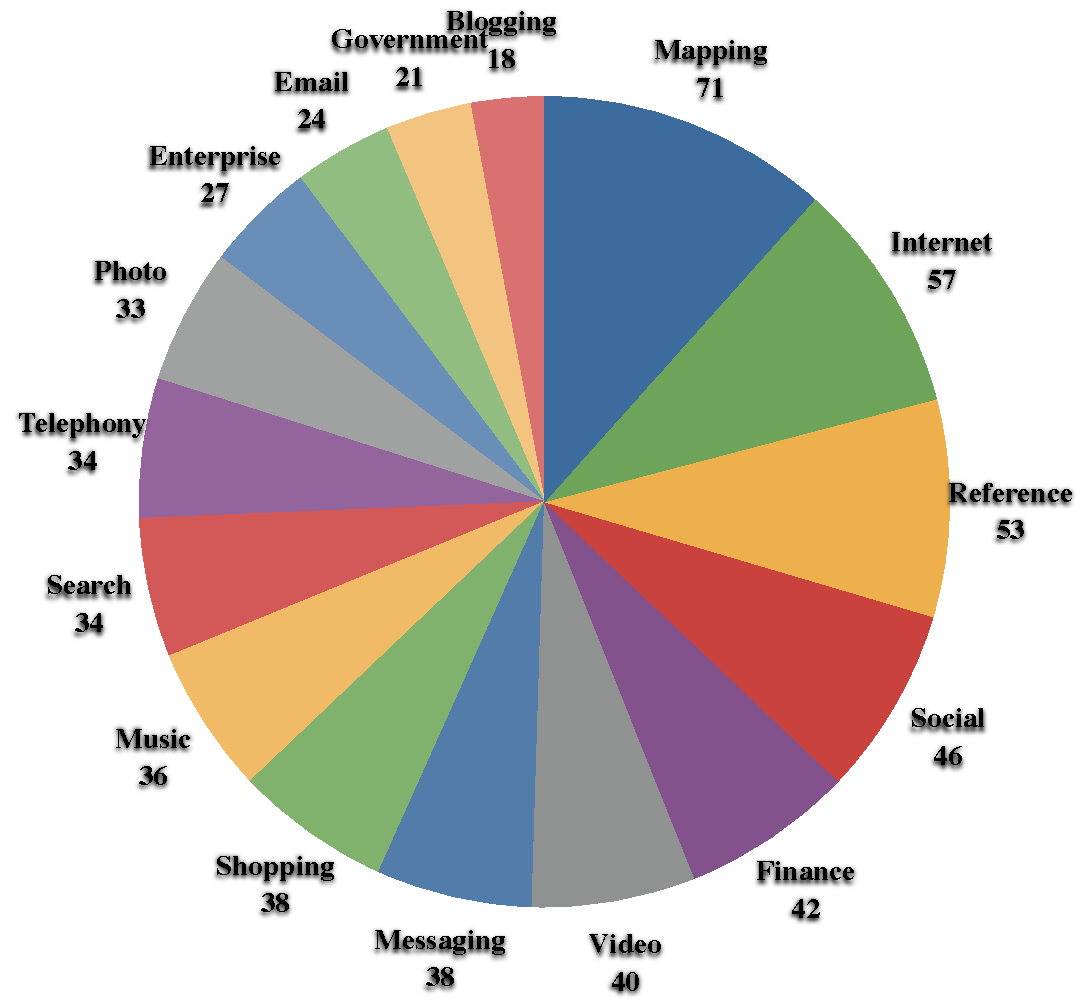
\includegraphics[width=.45\textwidth]{part1/pics/apis2008}\label{fig:api:2008}}
\hspace{3mm}
\subfloat[APIs, 2011]{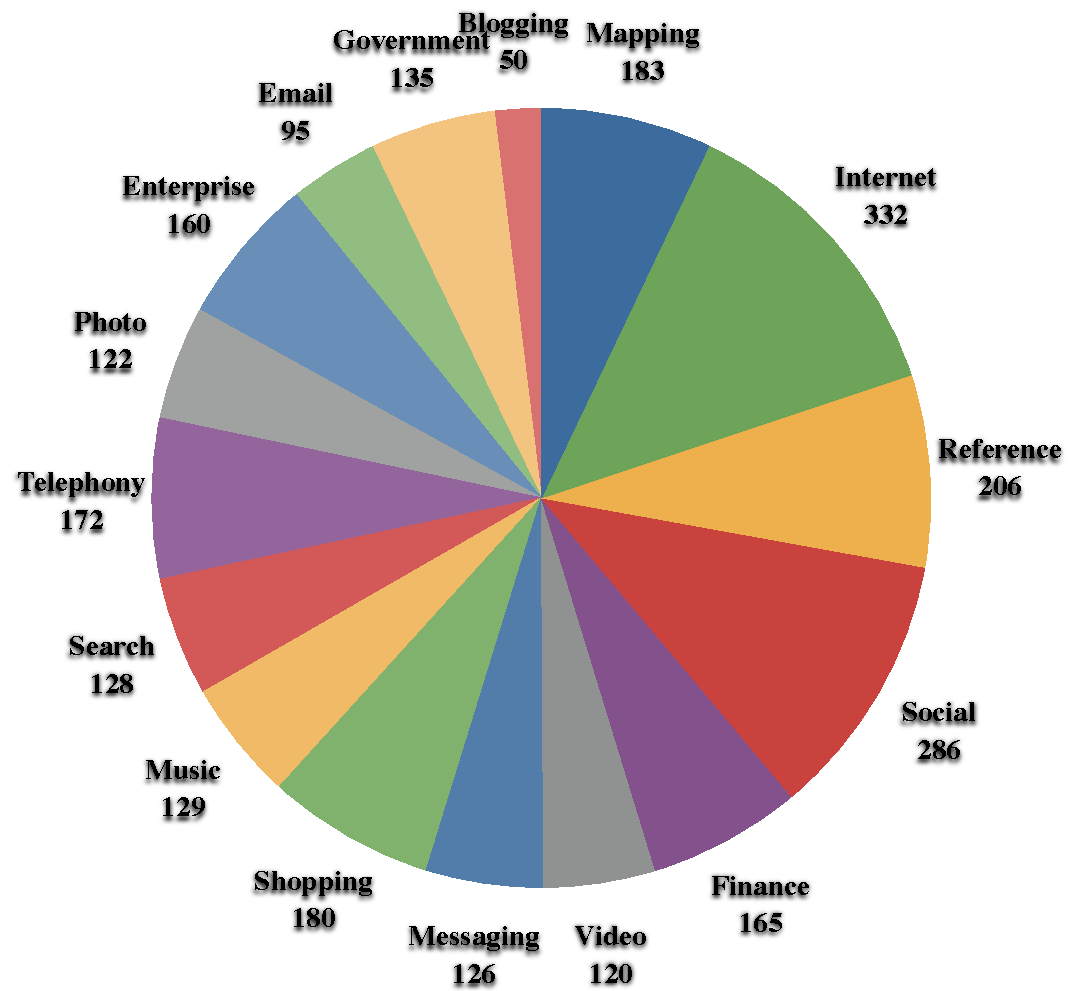
\includegraphics[width=.45\textwidth]{part1/pics/apis2011}\label{fig:api:2011}}
\end{center}
\caption{Data from~\cite{Domingue:2009} and actualized from ProgrammableWeb.com}
\label{fig:apis}
\end{figure}


{\bf Internet Of Services}\\
\label{subsec:ios}
Synergy is probably the best word to describe the \gls{ios} goal. Many services are now available on the Internet, such as hotel bookings, flight reservations or car rental. \gls{ios} aims to orchestrate the interactions of existing services to create new services more integrated, and dedicated to a task or a user. The goal is to create, for instance, a "Travels booking service" which aggregates the booking of a flight, hotel and car in a unique process.\\

Among all the "things" able to provide services, everyday life objects are also getting enriched with abilities to communicate through Internet-based technologies.\\

{\bf Internet Of Things}\\
\label{subsec:iot}
Stemming from the evolution of electronic devices, the \gls{iot} relates to an approach in which objects of everyday life have reached a sufficient level of maturity to interact one with each other. This interaction gives them the ability to act differently according to the situation 'sensed' with a stronger added value. Still in its infancy, the \gls{iot} is looking for software tools to develop and describe these interactions, as much as the services rendered.\\
Software components are quite suitable for virtualizing everyday life objects, and service-oriented computing is suitable for describing and implementing interactions. Software solutions developed in the future would probably merge both of these approaches. As long as it can be considered that a component offers services to other components, the collaboration of services and components produces promising results.\\

Information, devices and services are now able to communicate through the Internet, and render more and more integrated services to users. This strong integration requires all these services to be able to self-locate their dependencies, with no need for the user to set up technical properties (i.e.: server IP address, tcp port, etc...).\\

{\bf The Cloud}\\
\label{subsec:cloud}
Surfing on the service wave, hardware providers, software providers and others are offering more and more "things" as a service. Among others, \gls{saas} and \gls{paas} are the two main paradigms showing that everything can now be provided as a service.\\
The Cloud could be defined as the Internet of tomorrow. As everything is being served as a service, there is no more need to precisely locate services. Do you need a printer? Ask the cloud for the closest printer from you, and just use it. Might you need a lawyer? Ask the cloud for the best of them, and have a video-conference with him.\\
This approach makes it possible to obtain the hardware configuration you need, just-in-time, to run your software as a service. You will never know where your software is really run, but it will run in the cloud.\\

These principles are built on top of software architectures which basic elements are services or resources. Therefore, these approaches for building software are called Services-Oriented and Resource-Oriented architectures.

\subsubsection{Architectural principles}

In \cite{Papazoglou:2003}, M. Papazoglou defines Service-Oriented Architecture as "{\it a way of reorganizing software applications and infrastructure into a set of interacting services}". Services are able to describe themselves and realize computations for applications or other services, from a simple method execution to a complex business process. Services are offered by service providers which are responsible for the supply and support of their services. Clients of these services can be either applications or individuals, internally to the organization or from outside.\\
Possibly distributed over Internet, services must be {\it Technology Neutral} to be provided and used whatever the context, {\it Loosely coupled} to not rely on any specific context of use, and support {\it Location Transparency} by registering their location and description in directories such as UDDI, to allow clients to call the service regardless of its location.\\
%is a paradigm, an idea driving the way to develop software. Software services are rendering services to other services or individuals. If an application, or a software, uses services to achieve its goals, it is a service-based software.\\

%This section starts with some explanations about what is meant in this thesis by Service Oriented Architecture, and presents the S-Cube Network of Excellence, which funded this thesis. By the way, the last part of this section introduces to the new Internet of * paradigms.\\

{\bf SOA vs. WSOA}\\
In the Software Services community, service-oriented architecture is often used instead of web services-oriented architecture. However, there is a clear separation to respect between service-oriented architectures and web service.\\
Then, if a service is accessible through the Internet, this service is called web-service, and is a particular case of a service. Then service-oriented software can use this service as it would any other. \\
In conclusion, a service-based application does not necessarily use web-services and may even use no web service at all; there are other means of creating software based on services.\\

{\bf Web-Services}\\
A Web Service renders a service, using the Internet as a support. Web services are composed of methods that can be called by clients. Customers do not have to care about how the service is given and can just use it.\\

The use of Web Services is based on a "search and use" mechanism. Service providers are responsible for the registration of their services into a \gls{uddi} directory. When a client wants to use a service, he first searches in a service directory. Each registered service comes with a description, which helps clients in their service selection process. The real call to the service is made directly from the client to the server. Figure~\ref{fig:web-servce-archi} illustrates this mechanism.\\
\begin{wrapfigure}{r}{.5\textwidth}
%	\vspace{-0.5cm}
  \centering
  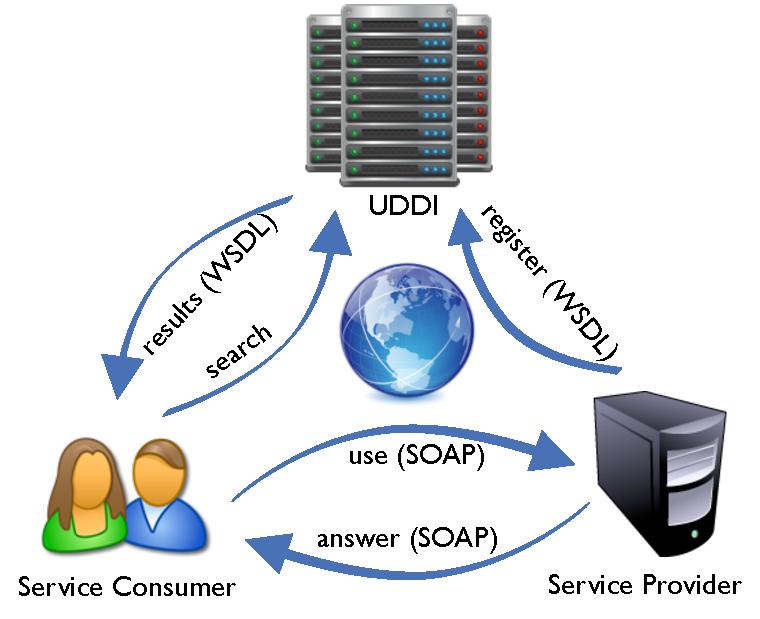
\includegraphics[width=.5\textwidth]{part1/pics/WSArchi.pdf}
  \caption{WebService Architecture}
  \label{fig:web-servce-archi}
%	\vspace{0.2cm}  
\end{wrapfigure}

Registrations and descriptions of services in the \gls{uddi} are based on a description language for web services called \gls{wsdl}. The description of a service informs users about the list of operations offered, parameters, and types of objects manipulated. Dynamic discovery and use of services are enabled this way.\\
Communications between clients, servers and \gls{uddi} instances use a unique carriage protocol called SOAP. SOAP has been based on XML descriptions in order to make use of HTTP, SMTP, and other application protocols as carriers.\\

Although this approach provides mechanisms for dynamic search and use with precise descriptions, the amount of data exchanged and the complexity of the SOAP message structure can become an issue. Resource-limited platforms may not be able to embed a SOAP parser, or have a power supply designed to send a large amount of communication data. To cope with this problem, Resource-Oriented Architectures have been proposed.\\


{\bf Resources-Oriented Architectures}\\
%\label{sec:rest}

In his doctoral dissertation in 2000 \cite{Fielding:2000}, Roy Fielding introduced the term and idea of Representational State Transfer (REST).\\
REST has been designed to lighten transfers of information through web-based communications. Instead of heavy serializations of concrete program objects, REST architectures are share representations of these objects using XML for instance. These representations handle all coherent and meaningful information for the request (resp. answer) to be processed by the server (or client). REST defines only four standard CRUD \cite{Yoder:1998} operations to manage resources.\\
{\bf GET} is to retrieve the resource pointed by the called url. {\bf POST} asks the server to add the information contained in the request (hence a resource representation) to the resources pointed at the requested url. The {\bf PUT} operation is used to create or entirely replace a resource, based on the representation contained in the request. Finally, {\bf DELETE} requests the server to delete the specified resource.\\
URLs of REST servers handle information about the resource concerned by a request. For instance, a GET request on a URL such as {\it http://myMedia.org/} would be answered with an XML representation of the entire media library; a POST containing information about a new book, called on the {\it http://myMedia.org/books} would result in the addition of this book in the book library. As a final example, a DELETE request on {\it http://myMedia.org/books/2517} should remove the book whose unique identifier is 2517 from the book collection.\\
For its transportation, REST was initially described in the context of HTTP but is not limited to that protocol. Supported by an application-level transfer protocol, REST is thus development-technology agnostic.\\


Thanks to the appearance of these two paradigms, ideas emerged about connecting software systems and everyday life objects. The presence of registries or auto-discovery mechanisms also led to an abstraction of the details of the physical location. These interconnections finally brought new paradigms known as the Internet of *. 


\subsubsection{OSGi}
\label{subsec:osgi}

OSGi~\cite{OSGI:r4} is an association created in 1999 aimed to provide facilities for software integration and development.
To achieve this task, the association released a set of specifications defining what any runtime implementation should do to reach a given service level. These specify which minimum set of services a runtime must offer to be compliant with the level.\\
In OSGi, services are given and contained in deployments units called {\it bundles}. Each bundle contains a {\it Manifest} file giving information about the runtime dependencies, the classes offered and some other information about what the bundle needs to run. Bundles can be installed, updated or removed at any time and their services can be started and stopped, with no need to restart the runtime platform.\\
Services are defined by Java interfaces (for Java runtime implementations), and are stored in the runtime context. Thus, any client on the platform who needs a service can search in the context registry for the service they need. Service method calls are locally handled inside a JVM, which makes this service-oriented runtime much faster than web service-based applications.\\

In OSGi, relations between bundles are never made explicit. Worse still, relations between bundles can be due to service dependencies that are just hard-coded and can only be changed by rebuilding and redeploying the bundle. In a static application, with few updates in time, this is not a real problem. Moreover, there are very few reflection primitives and thus, interactions between bundles can hardly be traced or even made explicit. OSGi do not address issues of interoperability, variability management nor safety and security. The registry mechanism is a good point concerning openness, and adaptations and evolutions of applications are simplified by the native lifecycle management of OSGi. In a word, OSGi lacks of a clear means of visualization of the architecture while running, but makes a very good base.\\

The table below is completed for each approach or tool, and presents strengths and weaknesses in a synthetic way. Individual tables are merged altogether in section~\ref{ch:summary} as a synthesis. \\
 \\
\begin{tabular}{ >{\centering}m{.13\textwidth}| >{\centering}m{.09\textwidth} >{\centering}m{.12\textwidth}| >{\centering}m{.10\textwidth} >{\centering}m{.20\textwidth}| >{\centering\arraybackslash}m{.15\textwidth}}
{\tiny Interoperability} & {\tiny Openness} & {\tiny Dynamic Adaptation} & {\tiny Static Evolution} & {\tiny Variability Management} & {\tiny Safety \& Security}\\
 \hline
  & + & + & + &  & \\ 
  \hline
\end{tabular}\\


\subsubsection{Enterprise Service Bus}

\gls{esb} refers to a business middleware family for service-oriented applications. This middleware acts as the only mediator of services in the enterprise, by providing a runtime environment for deploying business services. Legacy software can be integrated as services into the business service orchestration. These are declared as any other service, within the scope of the ESB runtime. The specifications have been successfully implemented in several frameworks such as OpenESB by SunMicrosystems, ServiceMix by Apache Foundation, or Petals by OW2.\\
\gls{jbi} or JSR 208 is an industrial Java standard developed to ease the integration of software systems over Service-Oriented Architectures. It uses an \gls{esb} as a basis to define a component model. It has been designed to reuse Java technologies such as WebServices, BPEL or JMS, and thus avoid new specific developments.  
In \gls{jbi}, components have an independent life-cycle and communicate through their services over normalized message middleware. In fact, this middleware acts as an abstraction layer for communications and eases the integration. \gls{jbi} components are split into two categories:\\
{\bf Service Engine Components} are directly hosted by the \gls{jbi} runtime environment, and are in charge of message processing, routing or orchestration of services. They cannot communicate outside of this scope.\\
{\bf Binding Components} expose or consume standard \gls{jbi} services, and perform the bindings with external non-standard software.\\
The packaging as components is described in the framework like this: service descriptions are encapsulated into Service Units, which are then encapsulated into deployable business components called Service Assemblies.\\
 
The message middleware makes \gls{jbi} a serious candidate in terms of interoperability of components. Openness is offered by the Binding Components, and evolutions are natively supported thanks to its service-oriented nature.
Besides its good properties, there is no clear separation between types and instances of services/components. Moreover, no introspection of services is offered and interconnections between components are not explicitly expressed, and sometimes even hard-coded inside the components.
This lack of clarity in the component interdependencies makes it impossible to dynamically replace components and/or reason about the system's state. This approach do not target the resolution of variability management or safety and security issues.\\
 \\
\begin{tabular}{ >{\centering}m{.13\textwidth}| >{\centering}m{.09\textwidth} >{\centering}m{.12\textwidth}| >{\centering}m{.10\textwidth} >{\centering}m{.20\textwidth}| >{\centering\arraybackslash}m{.15\textwidth}}
{\tiny Interoperability} & {\tiny Openness} & {\tiny Dynamic Adaptation} & {\tiny Static Evolution} & {\tiny Variability Management} & {\tiny Safety \& Security}\\
 \hline
 + & + &  & + &  & \\ 
  \hline
\end{tabular}\\


%\newpage
\subsection{Component models}
\label{sec:componentModelStateOfArt}
\vspace{0.3cm}


\subsubsection{Description}

Douglas McIlroy first introduced the notion of software component in 1968 at the NATO conference. This new paradigm defends a mass reuse of existing components and the creation of software as assemblies of components.\\
As described in \cite{Medvidovic:2000}, component models are made of three essential elements. A {\it Component} represents a computational unit and can realize an entire application or a single method. Components have a type and expose interfaces to collaborate with other components. This collaboration is enabled by component {\it Connectors}, in charge of the communication between the application's components. These connectors are typed and can have different behaviors, roles in the application, and can make use of various techniques to support components' interactions. Finally, a {\it Configuration} describes a particular assembly of components and connectors, and specifies the component-base software system.\\
The next section provides a brief list of component models.\\

\subsubsection{Darwin}

In~\cite{Georgiadis:2002} Ioannis Georgiadis and al. present a component model to describe self-organizing software architectures of distributed systems. In this model, components are defined by component types and can have multiple runtime instances. Instances can be statically specified at design time, or created on demand at runtime.
Usually, components provide and require services. The provision or requirement is made through typed ports. These types are specified by the interface of the service they offer.
Components are connected by their ports and the semantics of bindings is a classical service call. Obviously, port types have to be the same. Components can be assembled into composite components. Their specifications describe the instances used and how they are connected.\\
At runtime, component instances embed a view of the global configuration and a manager handling the architecture constraints, in charge of maintaining the configuration view synchronized with the system state.\\

The clear separation of types and instances is a plus. Runtime creation of instances can help in adapting the runtime to the environment. The configuration view synchronized with the runtime is a very interesting property. The use of Java class loading to change utility functions used by the policy manager is a good way to runtime evolution.\\
If the typing of ports is helpful to guarantee the consistency of an application model, the typing at the implementation level can act against the interoperability property, but enforce the safety of the system. Bindings have a clear semantic, but cannot use other communication links than the one they have been designed to use (Java RMI in this case). It is a limitation. The adaptation policies (in case of binding loss or component arrival for instance) are hard coded and distributed in each instance. Thus they cannot be easily changed at runtime.\\
\\
\begin{tabular}{ >{\centering}m{.13\textwidth}| >{\centering}m{.09\textwidth} >{\centering}m{.12\textwidth}| >{\centering}m{.10\textwidth} >{\centering}m{.20\textwidth}| >{\centering\arraybackslash}m{.15\textwidth}}
{\tiny Interoperability} & {\tiny Openness} & {\tiny Dynamic Adaptation} & {\tiny Static Evolution} & {\tiny Variability Management} & {\tiny Safety \& Security}\\
 \hline
  &  & + & + &  & + \\ 
  \hline
\end{tabular}\\


\subsubsection{Koala}

The Koala component model has been designed to handle the increasing diversity and complexity of embedded software and decrease development costs. Rob van Ommering and al. explain in ~\cite{RobVanOmmering:2000} that a way to achieve this is to model the software architecture and reuse existing software components rather than re-implementing the wheel. In their approach, a clear separation is made between component development and system configuration. It means that component developers cannot make any assumption about the context of use of each component and designers cannot change component behavior.\\
Components can require services provided by other component's ports.
A configuration describes an assembly of components. It handles the model of the application. To help in describing system assembly, Koala offers compound components in which  instances to be deployed and their interactions (bindings) are described. In this case, an action on a port of the compound component may have to be forwarded to internal components (e.g.: for initialization). To eliminate the ordering problem, Koala introduced {\it Modules} to handle one-to-many, many-to-one or many-to-many bindings. They are in charge of propagation and have a pre-defined treatment.\\

The clear separation between component development and assembly creation (for a particular application) is the key to success. Composition mechanisms are also welcome to cope with diversity management and promote the reuse of existing components to create value-added compound components. Here again, connection ports are typed and should conform to a specific interface. This is an advantage for securing the software but may cause problems in future evolutions, in terms of interoperability. Koala introduced modules to handle specific communications between components and act like a proxy. They could have gone a bit further by systematically using modules to specify each connection. This information could help in solving issues, or in specifying the system more precisely.\\
\\
\begin{tabular}{ >{\centering}m{.13\textwidth}| >{\centering}m{.09\textwidth} >{\centering}m{.12\textwidth}| >{\centering}m{.10\textwidth} >{\centering}m{.20\textwidth}| >{\centering\arraybackslash}m{.15\textwidth}}
{\tiny Interoperability} & {\tiny Openness} & {\tiny Dynamic Adaptation} & {\tiny Static Evolution} & {\tiny Variability Management} & {\tiny Safety \& Security}\\
 \hline
  &  &  & + & + & + \\ 
  \hline
\end{tabular}\\

\subsubsection{Fractal}

%Paragraph extracted from SEAA'10
Fractal~\cite{Bruneton:2006} is a modular and extensible component model to design, implement, deploy and reconfigure various systems and applications. Famous implementations of Fractal are Julia and AOKell (Java), Cecilia (C), FractNet (.NET) and FracTalk (SmallTalk).\\
The Fractal component model supports the definition of primitive and composite components. Each Fractal component consists of two parts: a controller, which exposes the component's interfaces, and content, which can be either a user class or other components in composite components. The model makes the bindings between the interfaces provided or required by these components explicit, as well as the hierarchic composition (including sharing).\\
Primitive components contain the actual code and composite components are only used as a mechanism to deal with a group of components as a whole, while potentially hiding some of the features of the subcomponents. Primitives are actually standard Java classes (in the Java distributions of Fractal) conforming to some coding conventions. Fractal does not impose any limit on the levels of composition, hence its name.\\
All interactions between components pass through their controller. The model thus provides two mechanisms to define the architecture of an application: bindings between interfaces of components, and encapsulation of a group of components into a composite. By default, Fractal proposes 6 controllers that may be present in components: Attribute, Name, Binding, Content, Lifecycle and Super Controller.\\
DigiHome\cite{Romero:2010} is a communication middleware built with Fractal. Its main objective is to offer a support for REST communications, and complex event processing, in a context of home automation.

Reflective execution platforms like Fractal or OpenCOM \cite{Blair:2004} do not provide a clear distinction between the reflection model and the reality. 
Modifying the reflection model implies a modification in the runtime. If this offers a means for adapting the runtime, there is no means to anticipate the effect of a reconfiguration, before actually executing it. Nor is there means to execute what-if scenarios to evaluate different possible configurations, etc. This point is a drawback from a safety viewpoint.
This lack of an explicit and independent reflection model imposes that most of the verifications must be carried out while reconfiguring. Pre-condition on reconfiguration actions, as proposed by L\'eger \cite{Leger:2007}, are checked and roll-backs are performed if something goes wrong.
In addition, component models such as Fractal are slightly opaque with respect to the outside world, making openness and reuse by third party applications complicated if not anticipated in advance. Lastly, the dynamicity of an application running over Fractal is compromised, because the deployment of new component' types can not be carried out without restarting.\\
 \\
\begin{tabular}{ >{\centering}m{.13\textwidth}| >{\centering}m{.09\textwidth} >{\centering}m{.12\textwidth}| >{\centering}m{.10\textwidth} >{\centering}m{.20\textwidth}| >{\centering\arraybackslash}m{.15\textwidth}}
{\tiny Interoperability} & {\tiny Openness} & {\tiny Dynamic Adaptation} & {\tiny Static Evolution} & {\tiny Variability Management} & {\tiny Safety \& Security}\\
 \hline
  &  & + &  &  &  \\ 
  \hline
\end{tabular}\\


\newpage
\subsection{Component Models for SOA}

\subsubsection{Description}

By nature, Service-Oriented software is dynamic and its architecture is not always easy to figure out. Indeed, the services used and the connections between software elements are never known prior to the execution because of the late binding principle. The late binding principle relates to the fact that a service to be used is searched and selected just before its call. Component models for \gls{soa} have been invented to try to make the description of this kind of application more explicit. They merge well-known software component techniques with new services ideas, and tend to conciliate the best of each approach.\\

Components, as defined by component models, provide services to other components through their ports. Components' ports are defined by an API. Services, from service-oriented architectures are intended to be used in orchestrations to create value-added applications.\\
Since both of these concepts offer services, new component models have been designed to merge both paradigms. This section presents some famous implementations of these component models.\\

\subsubsection{SCA}

\gls{sca}\footnote{http://www.osoa.org/} provides a component model for both the composition of services and for the creation of service components.
\gls{sca} is a model that aims to encompass different programming languages, frameworks and environments commonly used to build components and services, such as Web Services, Messaging systems and \gls{rpc} for communication purposes. Its goal is to setup a single and common way to access and assemble service-based applications.\\
\gls{sca} can be presented through four major parts of the specification.\\

{\bf Specifications}\\
\par {\bf Assembly} defines how components are packaged as services and how they can be combined into composites that perform a particular task.
Composite components can be used as classical service components, which simplifies their reuse. Assembly in \gls{sca} also defines how components and composites are connected. Functional service properties, such as data encryption, or authentication, are described outside the service business code, which saves developers' valuable time. Indeed, it enables the modification of the connections or the properties, without changing the business code.
\par {\bf Client and Implementation Model} defines how services are packaged and accessed in various languages. API implementations in Java, BPEL, C++, Javascript or the Spring Framework, offer means to package a service or access any \gls{sca} service. For development concerns, it means that there is only one interface and packaging method to learn to provide and use any \gls{sca} service. This interface makes it possible to access to the component using Web services, JMS, JCA and EJBs natively. Here again, service properties are described outside the code, to make changes much easier.
\par {\bf Policy Framework} is aimed at offering means for the definition of security, authentication, quality of service, and other important policies of a service. In fact, the \gls{sca} Policy Framework makes use of the WS-Policy and WS-Policy Framework open standards, as a support to describe policies. This way, descriptions of policies such as "any data sent to this service must be encrypted" or "the user of this service must be authenticated" are made available. Here again, policies can be defined outside the business code of the service.
\par {\bf Bindings} specify the mechanisms that can be used to access or connect a component. Bindings can be implemented using Web services, JMS, JCA, EJBs or any other communication way. Keeping the consistency of the approach, bindings are defined outside the component business code.\\

SCA is a standard, a set of definitions describing how such a system should behave. Thus, it imposes certain types of implementation, in order to guarantee the presence of mechanisms for openness, evolution or remote control.\\
\\
\begin{tabular}{ >{\centering}m{.13\textwidth}| >{\centering}m{.09\textwidth} >{\centering}m{.12\textwidth}| >{\centering}m{.10\textwidth} >{\centering}m{.20\textwidth}| >{\centering\arraybackslash}m{.15\textwidth}}
{\tiny Interoperability} & {\tiny Openness} & {\tiny Dynamic Adaptation} & {\tiny Static Evolution} & {\tiny Variability Management} & {\tiny Safety \& Security}\\
 \hline
  & + &  & + &  & + \\ 
  \hline
\end{tabular}\\


\subsubsection{FraSCAti}

FraSCAti~\cite{Melisson:2010} is an implementation of the SCA specifications. It is certainly the closest approach to what is required. Components can be composed into composite components. Communications between components are made using services and several communication media can be used. These elements make FraSCAti a serious candidate to address openness and remote control concerns.\\
In the past months, efforts have been spent on integrating FraSCAti and OSGi, which have improved its faculties of evolution. In terms of interoperability, FraSCAti offers mechanisms for the connection of services, but does not directly address the integration of smart devices. Thus, interoperability of components in our context is still compromised by the use of APIs, for the definitions of services rendered and required, by ports. If two components have not been designed to be connected, an ad-hoc connector has to be created.\\
The FraSCAti script tool enables reconfiguration and adaptation of component assemblies. But adaptations are limited to the manipulation of binding and component instances, whose types are available on the platform. New instances can be created, new bindings can be set, but no new types can be installed using FraSCAti Script.\\
The variability of FraSCAti itself is managed using a Software Product Line(SPL). Each runtime instance of FraSCAti is a product of the SPL. Thus, features of FraSCAti can be deployed on demand. However, this variability management concerns only the internal features of FraSCAti, and an external tool is still required to handle the variability of applications made with FraSCAti.\\
\\
\begin{tabular}{ >{\centering}m{.13\textwidth}| >{\centering}m{.09\textwidth} >{\centering}m{.12\textwidth}| >{\centering}m{.10\textwidth} >{\centering}m{.20\textwidth}| >{\centering\arraybackslash}m{.15\textwidth}}
{\tiny Interoperability} & {\tiny Openness} & {\tiny Dynamic Adaptation} & {\tiny Static Evolution} & {\tiny Variability Management} & {\tiny Safety \& Security}\\
 \hline
 + & + &  & + &  & + \\ 
  \hline
\end{tabular}\\

\subsubsection{iPOJO}
iPOJO~\cite{Escoffier:2007} is the Apache service-oriented component runtime built on top of OSGi \gls{soa} platforms. iPOJO is the natural evolution of the Service Binder mechanism introduced by Cervantes et al. in~\cite{Cervantes:2004}. The iPOJO framework merges the advantages of component- and service-oriented paradigms. Specifically, application functionalities are implemented following the component paradigm. Each component is fully encapsulated, self-sufficient, and provides server and client interfaces as services. An iPOJO component is actually managed by a reusable container, which provides common middleware functionalities. Each component container can be configured with a different set of middleware services.\\
The iPOJO component model focus on providing management facilities for pervasive applications based on component model, and a service-oriented runtime. This general purpose component model for service oriented architectures provides a solid base for domain specific extensions and developments.
 \\
\begin{tabular}{ >{\centering}m{.13\textwidth}| >{\centering}m{.09\textwidth} >{\centering}m{.12\textwidth}| >{\centering}m{.10\textwidth} >{\centering}m{.20\textwidth}| >{\centering\arraybackslash}m{.15\textwidth}}
{\tiny Interoperability} & {\tiny Openness} & {\tiny Dynamic Adaptation} & {\tiny Static Evolution} & {\tiny Variability Management} & {\tiny Safety \& Security}\\
 \hline
  & + & + & + &  & \\ 
  \hline
\end{tabular}\\


\newpage
\section{Domain-specific approaches}
\label{sec:domainSpecificApproaches}

General purpose approaches make it possible to design and implement software solutions for many problems. But this flexibility comes with a complexity due to the knowledge required to be able to develop or simply use these approaches.\\

Domain-specific approaches tend to reduce this complexity to a minimum, by providing tools on top of general purpose approaches adapted to a specific domain of use. In this section, several tools built upon this principle are reviewed to list their advantages and disadvantages.

\subsection{Description}
\label{sec:mdeEtDSL}


\gls{mde} is an approach that promotes the use of an abstract representation of a piece of software, before its actual realization. From this abstract view, tools and methods make it possible to automate the final software generation, tests and validations across pre-defined requirements. Models are human understandable representations of reality. They can handle information about structure, data exchange, communication links, or some building constraints of a piece of software.\\
\gls{dsl} are another means of abstraction and description of software systems. Dedicated to a specific domain, they can be graphical, textual or both. They are designed to restrict the concepts manipulated to the ones from the application domain. This approach makes it easier for domain specialists to express a software system architecture and behavior, by using their own terminology.\\

The goal of these tools is to provide a sufficient level of abstraction to make software development easier, more flexible, with an enhanced level of reliability, and shorter time-to-market.\\
The rest of this section presents several approaches built around the concepts of \gls{mde} and/or \gls{dsl}, that simplify the creation of applications in the domain of home automation and/or pervasive computing.\\


\subsection{Projects}

\subsubsection{uMiddle}
Nakazawa et al propose a framework that bridges remote smart spaces called D-uMiddle in~\cite{Nakazawa:2007}. This makes it possible for a device to interact with another, over the Internet. This is made available by four distinct features of D-uMiddle. Firstly, a local mapper mechanism abstracts sensor nodes into common representations. Secondly, a mechanism translates data transmission protocols from a node-specific one to a D-uMiddle common one. Thirdly, a remote mapper mechanism creates proxies of sensor nodes from remote smart spaces in the local space. Fourthly, a transport module enables devices to receive data over IPv4 NATs network. The consumer devices, as a result, can use sensor nodes in remote smart spaces without depending on their own protocols and semantics, and without being burdened by the complicated IPv4 NATs.\\

D-uMiddle brings a solution for connecting remote smart spaces, with no need for a developer to care about transportation. Remote control of equipment is thus made possible for free. Nevertheless, it does not supply tools to handle variability, adaptation or evolution of a deployed system, and nothing is specified about the securization of the connection.\\
 \\
\begin{tabular}{ >{\centering}m{.13\textwidth}| >{\centering}m{.09\textwidth} >{\centering}m{.12\textwidth}| >{\centering}m{.10\textwidth} >{\centering}m{.20\textwidth}| >{\centering\arraybackslash}m{.15\textwidth}}
{\tiny Interoperability} & {\tiny Openness} & {\tiny Dynamic Adaptation} & {\tiny Static Evolution} & {\tiny Variability Management} & {\tiny Safety \& Security}\\
 \hline
  &  &  &  &  & \\ 
  \hline
\end{tabular}\\

\subsubsection{SOPRANO}
SOPRANO (Service-Oriented Programmable Smart Environments for Older Europeans) was an Integrated European Project, which successfully ended in April 2010. Its main achievement was the release of openAAL~\cite{Wolf:2010}, a framework built on top of an OSGi execution platform. OpenAAL helps in getting information from devices, and acting on them from a higher level of abstraction. Its framework integrated a context manager, able to give a virtual view of all devices, a process manager in charge of making decisions for any change in the context, and a composer, dealing with the actual services for interaction with the real environment.\\

OpenAAL proposes a solution to efficiently built applications ready to evolve with needs and able to adapt to changes in context. However, no attention is paid to the variability management, remote control or interoperability of devices. Nothing is said about safety of security.\\
 \\
\begin{tabular}{ >{\centering}m{.13\textwidth}| >{\centering}m{.09\textwidth} >{\centering}m{.12\textwidth}| >{\centering}m{.10\textwidth} >{\centering}m{.20\textwidth}| >{\centering\arraybackslash}m{.15\textwidth}}
{\tiny Interoperability} & {\tiny Openness} & {\tiny Dynamic Adaptation} & {\tiny Static Evolution} & {\tiny Variability Management} & {\tiny Safety \& Security}\\
 \hline
  &  & + & + &  & \\ 
  \hline
\end{tabular}\\


\subsubsection{Ga\"ia Framework}
Ga\"ia~\cite{Roman:2002} is presented as a meta-operating system for ubiquitous computing, built on top of a classical operating system. Its goal is to detach itself from the heterogeneity and complexity associated to ubiquitous environments. Ga\"ia is composed of a Kernel, responsible for the runtime management of applications and a Framework to build these applications. An application runs in an Active Space, a physically-limited space where services and devices are available for ubiquitous computing.\\
Each Ga\"ia instance is specifically configured for the active space it manages. To allow for describing Ga\"ia applications for several active spaces, Olympus\cite{Ranganathan:2005} proposes a high-level DSL working with virtual entities. From an Olympus application model, the underlying Ga\"ia OS takes responsibility for mapping each virtual entity to a service, or device, available in the active space.\\
It has been implemented in CORBA and can be ported to other communication middleware architectures such as SOAP or RMI.\\

The interoperability of services and devices is ensured by the common set of basic services. Adaptations and evolutions are made possible by the Component Management Core of Ga\"ia which can dynamically load, transfer, create or destroy components or applications. Remote control is made available by the underlying CORBA platform, in the implementation described. Variability management of components or applications, safety and security, and openness of the solution are not targeted by this work.\\
\\
\begin{tabular}{ >{\centering}m{.13\textwidth}| >{\centering}m{.09\textwidth} >{\centering}m{.12\textwidth}| >{\centering}m{.10\textwidth} >{\centering}m{.20\textwidth}| >{\centering\arraybackslash}m{.15\textwidth}}
{\tiny Interoperability} & {\tiny Openness} & {\tiny Dynamic Adaptation} & {\tiny Static Evolution} & {\tiny Variability Management} & {\tiny Safety \& Security}\\
 \hline
 + &  & + & + &  &  \\ 
  \hline
\end{tabular}\\


\subsubsection{DiaSuite}
DiaSuite\footnote{http://phoenix.inria.fr/projects/diasuite} is a software tool suite designed to ease the creation of pervasive and/or distributed applications. DiaSuite~\cite{CASSOU:2010} is composed of several elements. DiaSpec is the \gls{adl} of the suite, used to describe the applications at a convenient level of abstraction. From this description, DiaGen automates the code generation of the application, and DiaSim provides the support for the test, simulation and validation of the generated application. As an example, Bertrand et al. present in \cite{BERTRAN:2010} how they used the SIP protocol as a generic communication bus for a pervasive application developed with DiaSuite tools.\\
This tool suite has been augmented with Pantagruel\footnote{https://pantagruel.bordeaux.inria.fr/}, a visual \gls{dsl} created to support the development of pervasive applications. A first step when using Pantagruel aims at defining the entities involved in the future application domain. In a second step, entities of the application are orchestrated in order to define the logic of the application. A last step generates an application code, compatible with the DiaSuite tools. Details about this tool are available in \cite{DREY:2009}.\\


These tools meet the demands of a tool chain to develop pervasive applications from a high-level description. Code generation and the simulation environment are very good tools to improve the efficiency of the development process and the reliability of the code, as much as facing the variability of solutions. Designed to ease the development of pervasive applications, these tools do not address issues about variability management, application evolutions or adaptations.\\
\\
\begin{tabular}{ >{\centering}m{.13\textwidth}| >{\centering}m{.09\textwidth} >{\centering}m{.12\textwidth}| >{\centering}m{.10\textwidth} >{\centering}m{.20\textwidth}| >{\centering\arraybackslash}m{.15\textwidth}}
{\tiny Interoperability} & {\tiny Openness} & {\tiny Dynamic Adaptation} & {\tiny Static Evolution} & {\tiny Variability Management} & {\tiny Safety \& Security}\\
 \hline
 + & + &  &  & + & + \\ 
  \hline
\end{tabular}\\


\subsubsection{Habitation}
Habitation is a methodology, a set of tools to address the specific requirements of home automation application development and design. In \cite{Jimenez:2009}, Jimenez et al. describe how the combination of a \gls{dsl}, and an \gls{mde} approach eases the creation of solutions in this domain. Habitation proposes three main tools. A catalog of functional units centralizes elements that can be reused in various applications. Home automation devices are composed of several functional units. The second tool is a workspace in which elements of the catalog can be placed to define a specific application. Called the application view, this tool aims to provide tools for the assembly work and make it accessible for non-domain experts. The last tool is a kind of engine, which translates from the model and \gls{dsl} description, to a technology-specific configuration file.\\


The approach proposed by Habitation is very promising and sounds helpful in providing non-expert users with tools having a sufficient level of abstraction to be user friendly. However, Habitation only addresses pre-deployment design issues and does not deal with issues such as evolutions, adaptations and safety and security issues. Such as DiaSuite, Habitation remains an good approach to face the variability issue, while improving the efficiency of the development process.\\
\\
\begin{tabular}{ >{\centering}m{.13\textwidth}| >{\centering}m{.09\textwidth} >{\centering}m{.12\textwidth}| >{\centering}m{.10\textwidth} >{\centering}m{.20\textwidth}| >{\centering\arraybackslash}m{.15\textwidth}}
{\tiny Interoperability} & {\tiny Openness} & {\tiny Dynamic Adaptation} & {\tiny Static Evolution} & {\tiny Variability Management} & {\tiny Safety \& Security}\\
 \hline
 + &  &  &  & + & \\ 
  \hline
\end{tabular}\\


\subsubsection{Wired Application Description Language}
Wired Application Description Language(WADL) is a language designed to ease the description of dynamic applications, and provide an explicit view of the relations between elements. In \cite{Cervantes:2008} authors present how WADL has been used in the creation of a dynamic sensor-based application.\\
WADL has been implemented on OSGi(see section~\ref{subsec:osgi}) and relies on the WireAdmin service offered by the execution platform. In this implementation, wires between producers of information and consumers are dynamically created or deleted, according to the elements available in the system. Wires are specified by two filters. Each filter is used to make a selection among all available services, and capture producers' (or consumers') services required for the wire.\\

WADL provides a tool to explicit the architecture of dynamic applications, which is often difficult to extract because of the runtime evolutions. By nature, this approach copes with the adaptation requirement. The interoperability is realized by the use of a Producer/Consumer pattern. Evolution is supported by the filters that can be flexible enough to admit future evolutions. Issues on openness, variability management and safety and security are not treated in this approach.\\
\\
\begin{tabular}{ >{\centering}m{.13\textwidth}| >{\centering}m{.09\textwidth} >{\centering}m{.12\textwidth}| >{\centering}m{.10\textwidth} >{\centering}m{.20\textwidth}| >{\centering\arraybackslash}m{.15\textwidth}}
{\tiny Interoperability} & {\tiny Openness} & {\tiny Dynamic Adaptation} & {\tiny Static Evolution} & {\tiny Variability Management} & {\tiny Safety \& Security}\\
 \hline
 + &  & + & + &  & \\ 
  \hline
\end{tabular}\\


\subsubsection{PervML}
Mu\~nos et al. present PervML in~\cite{Munoz:2006a,Munoz:2006b} in the context of the management of a pervasive meeting room. PervML is a Model Driven Approach designed to ease the development of pervasive systems. This language separates the analyst's view, describing the requirements of the system at a high level of abstraction, from the architect's view, where devices and implementation details are specified.\\
This abstract model of the system is then used in a tool chain which ends up with an executable OSGi(see section~\ref{subsec:osgi}) code. This tool chain, detailed in \cite{Munoz:2006}, firstly transforms the platform independent PervML model to an OSGi dependent model, and then generates the executable Java code.\\
PervML and the associated generation tool chain are available as a plugin for Eclipse \cite{Cetina:2007}.\\
In \cite{Serral:2010a}, authors explain how they introduced system evolution capabilities to adapt the generated systems to changes in user behavior. Their solution uses a context model, to detect specific situations, and a task model describing the jobs to be executed for each detected context.\\

PervML offers a suitable solution. Developed to be executed on an OSGi platform, it naturally offers adaptation, evolution, openness and interoperability mechanisms. As presented in \cite{Cetina:2009}, PervML also targets the variability management issue. So far, a drawback of this approach is that people have to be familiar with UML to model a pervasive application. Also, the use of a pre-defined set of service interfaces described in the framework may become a barrier for the flexibility of the solution. Safety and security issues are not addressed by this work.\\
\\
\begin{tabular}{ >{\centering}m{.13\textwidth}| >{\centering}m{.09\textwidth} >{\centering}m{.12\textwidth}| >{\centering}m{.10\textwidth} >{\centering}m{.20\textwidth}| >{\centering\arraybackslash}m{.15\textwidth}}
{\tiny Interoperability} & {\tiny Openness} & {\tiny Dynamic Adaptation} & {\tiny Static Evolution} & {\tiny Variability Management} & {\tiny Safety \& Security}\\
 \hline
 + & + & + & + & + & \\ 
  \hline
\end{tabular}\\




\subsubsection{AutoHome}

In~\cite{Bourcier:2011}, Bourcier et al. present AutoHome as an autonomic management framework for pervasive home applications. AutoHome is described as a middleware that extends the iPOJO component model, to create a framework to host autonomic home applications. Using this approach, authors aim to separate the design and development of the application itself, from autonomic management components. They aim to enable the development of autonomic management functions, ease their integration with the applications, and finally, deploy the resulting autonomic application on execution environments shared with other applications. As a consequence, an application on top of AutoHome has the following architectural elements: middleware offering an autonomic service-oriented component and a context facility, a runtime that includes monitoring and reconfiguration abilities, a set of service-oriented applications which represent pervasive components to be autonomously managed, and a set of managers organized in a hierarchy.\\

AutoHome makes it possible to include, within the application itself, specialized components that monitor and react on component or platform events.
However, this solution does not seem to offer means for variability management, or interoperability between components, and does not consider safety or security aspects.\\
 \\
\begin{tabular}{ >{\centering}m{.13\textwidth}| >{\centering}m{.09\textwidth} >{\centering}m{.12\textwidth}| >{\centering}m{.10\textwidth} >{\centering}m{.20\textwidth}| >{\centering\arraybackslash}m{.15\textwidth}}
{\tiny Interoperability} & {\tiny Openness} & {\tiny Dynamic Adaptation} & {\tiny Static Evolution} & {\tiny Variability Management} & {\tiny Safety \& Security}\\
 \hline
  & + & + & + &  & \\ 
  \hline
\end{tabular}\\


\subsubsection{WComp}

WComp\cite{Ferry:2011uq,Tigli:2009} is a component model designed to support ubiquitous computing. It tries to address issues introduced by the mobility of devices, their heterogeneity and the dynamicity of the execution environment in this domain. To cope with these problems, WComp federates three paradigms. Event-Based Web Services, firstly, that plays an important role in facing the heterogeneity of devices, as much as the dynamicity, the extensibility and scalability of a ubiquitous system. Secondly, a Lightweight component-model (called SLCA) is introduced and used to compose event-based Web services, and expose a new service. The third paradigm used concerns the adaptation and makes use of the Aspect of Assembly concept. These aspects define adaptations on assemblies using structural descriptions. Adaptation are thus not specific to particular service assemblies and can be composed.\\

WComp offers several mechanism for adaptations, evolutions and interoperability,  and does not seem to address openness, variability management and safety or security concerns. Finally, it looks like the type system of the components rely on the implementation language type system, which can limit the reuse and interoperability.\\
 \\
\begin{tabular}{ >{\centering}m{.13\textwidth}| >{\centering}m{.09\textwidth} >{\centering}m{.12\textwidth}| >{\centering}m{.10\textwidth} >{\centering}m{.20\textwidth}| >{\centering\arraybackslash}m{.15\textwidth}}
{\tiny Interoperability} & {\tiny Openness} & {\tiny Dynamic Adaptation} & {\tiny Static Evolution} & {\tiny Variability Management} & {\tiny Safety \& Security}\\
 \hline
 + &  & + & + &  & \\ 
  \hline
\end{tabular}\\

\subsubsection{Niagara}

NiagaraAX is a software framework and a development environment that leverage the accessibility of a device toward an Internet access. 
The normalization proposed by NiagaraAX of the behavior and data gathered from several devices, enables the implementation of seamless, Internet-connected, web-based systems, whatever their manufacturer or communication protocol. This normalization has been enabled by the Niagara's unique, patented component model that transforms the data from diverse external systems into uniform software components.
These components share the foundation for building applications to manage and control the devices.\\

NiagaraAX eases the creation of applications integrating services and devices, by providing a framework for the development of drivers and applications. Built as a service-oriented architecture, this framework promotes the interoperability of devices and openness of solutions through Internet-based communications. NiagaraAX does not target issues about adaptations of the software or its evolution at runtime. Safety and security are not part of this work.\\
 \\
\begin{tabular}{ >{\centering}m{.13\textwidth}| >{\centering}m{.09\textwidth} >{\centering}m{.12\textwidth}| >{\centering}m{.10\textwidth} >{\centering}m{.20\textwidth}| >{\centering\arraybackslash}m{.15\textwidth}}
{\tiny Interoperability} & {\tiny Openness} & {\tiny Dynamic Adaptation} & {\tiny Static Evolution} & {\tiny Variability Management} & {\tiny Safety \& Security}\\
 \hline
 + & + &  &  &  & \\ 
  \hline
\end{tabular}\\





\chapter{Synthesis}
\label{ch:summary}

Scientific literature abounds with proposals using different approaches to cope with interoperability, adaptation or remote control concerns in several applications.\\
Generally, service-based propositions sound helpful in targeting the interoperability of devices, but clearly lack description of the running application once deployed. They bring essential ideas to properly handle the arrival and departures of elements, since a service can be started and stopped at any time.\\
Component-based architectures provide an ideal abstraction level that meets the requirements for a virtual representation of home automation devices. 
However, the specialized interfaces used as descriptions for ports, may prevent the realization of unpredicted connections.\\
Using components for \gls{soa} is certainly the best approach for our concerns. Bridging components and services makes the benefits balance out the drawbacks of each.\\
Transversally, model-driven engineering methods and techniques come with a lot of tools for virtual element manipulations. They seem handy for runtime management of devices, for the description of software systems and for variability management.\\


\begin{table}[h!]
\begin{tabular}{cm{.23\textwidth}|| >{\centering\arraybackslash}m{.06\textwidth}| >{\centering\arraybackslash}m{.07\textwidth}| >{\centering\arraybackslash}m{.09\textwidth}| >{\centering\arraybackslash}m{.08\textwidth}| >{\centering}m{.11\textwidth}| >{\centering\arraybackslash}m{.08\textwidth}|}
 & & {\tiny Interop.} & {\tiny Openness} & {\tiny Dynamic Adaptation} & {\tiny Static Evolution} & {\tiny Variability Management} & {\tiny Safety \& Security}\\
 \hline\hline
 \multirow{7}{7mm}{\begin{sideways}\parbox{25mm}{\small\centering Generic Approaches}\end{sideways}}
 %&{\small Hydra} 		& + & + & + &  &  & \# \\
 &{\small OSGi~\cite{OSGI:r4}}				&  & + & + & + &  &  \\ 
 &{\small ESB~\cite{Chappell:2004}}								& + & + &  & + &  &  \\
 \cline{2-8}%\hline
 %\multirow{3}{7mm}{\begin{sideways}\parbox{13mm}{\centering \tiny Component Models}\end{sideways}}
 &{\small Darwin~\cite{Georgiadis:2002}}		&  &  & + & + &   & + \\ 
 &{\small Koala~\cite{RobVanOmmering:2000}}	&  &  &   & + & + & + \\
 &{\small Fractal~\cite{Bruneton:2006}}		&  &  & + &   &   &  \\
 \cline{2-8}%\hline
 %\multirow{2}{7mm}{\begin{sideways}\parbox{12mm}{\centering \tiny Component Models for SOA}\end{sideways}}
 &{\small SCA~\cite{sca:specs}}				&   & + &  & + &  & +\\
 &{\small FraSCAti~\cite{Melisson:2010}}	 	& + & + & + & + &  & + \\
 &{\small iPOJO~\cite{Escoffier:2007}}		&  & + & + & + &  &  \\
 \hline\hline
 \multirow{9}{7mm}{\begin{sideways}\parbox{30mm}{\small\centering  Domain-Specific Approaches}\end{sideways}} 
 &{\small uMiddle~\cite{Nakazawa:2007}}		&  &  &  &  &  &  \\
 &{\small SOPRANO~\cite{Wolf:2010}}			&  &  & + & + &  &  \\
 &{\small Ga\"ia~\cite{Roman:2002}}			& + &  & + & + &  &  \\
 &{\small Dia Suite~\cite{CASSOU:2010}}		& + & + &  &  & + & + \\
 &{\small Habitation~\cite{Jimenez:2009}}	& + &  &  &  & + &  \\
 &{\small WADL~\cite{Cervantes:2008}}		& + &  & + & + &  &  \\
 &{\small PervML~\cite{Munoz:2006a}}			& + & + & + & + & + &  \\
 &{\small AutoHome~\cite{Bourcier:2011}}		&  & + & + & + &  &  \\
 &{\small WComp~\cite{Ferry:2011uq}}			& + &  & + & + &  & \\
 &{\small Niagara~\cite{Tridium:2008}}		& + & + &  &  &  &  \\
 \hline
\end{tabular}
\caption{Summary of existing approaches}
\label{tab:summaryOfApproaches}
\end{table}




Table~\ref{tab:summaryOfApproaches} summarizes the advantages and the disadvantages of the approaches described in the State-of-the-art Review.\\


\section{Good properties identified}

All throughout existing approaches, some good design properties have been collected. These properties are not sufficient to address all our issues, but are still necessary to properly cope with challenges. Some of these properties had been suggested in~\cite{Nain09a} to cope with the requirements.\\

{\bf Reflexive Model}\\
Coming from the \gls{mde} domain, the goal is to obtain and keep synchronized, an explicit and independent model reflecting the architecture living at runtime. This model makes it possible to reason about the application state and perform any required operation with no risk for the running system due to decoupling. An adaptation engine, for instance, is thus able to select, test and validate an adaptation scenario on the model, before actually performing the adaptation on the running system~\cite{Leger:2007}.
Component-based execution systems often offer introspection capabilities making it possible to build this kind of model.\\

{\bf Externalized coupling}\\
For a system to be handled in the right way, interactions between its composing elements have to be explicit. Component Models and \gls{dsl} offer a means of description for these interactions. A clear and explicit description of the relation between components gives a better understanding, and makes the analysis of the system much more accurate. It leads to better adaptation decisions, taking into account concurrency problems or dependency cycles for instance.\\
Moreover, this externalization and the description of interactions and dependencies enforce the independence of the elements composing the system. It also improves the flexibility of the system, thanks to the possibility of modifying of the resolution and connection policies with no need to deal with business components.\\

{\bf Hot deployment}\\
The possibility for a service to be dynamically deployed or removed during the runtime of a system is an essential principle to be considered while dealing with flexibility, adaptations and evolutions. The execution platform must therefore, support dynamic deployments and adaptations of the application during runtime with no restart. This is a basic facility offered by \gls{soa} execution environments.\\

{\bf Loose coupling}\\
Component Models promote the loose coupling principle, meaning that all components must have independent life cycles, and no execution dependencies with each other (in term of libraries). This is necessary to enable and ease the replacement of elements in a system. Indeed, inter-component dependencies may imply a huge alteration of the system to replace a single component, just because it depends on other components. It may also result in a more complex computational process of impacts for a change, or worse, an impossibility for the system to evolve or be adapted.\\

{\bf Openness}\\
Interoperability and openness to third party applications/contributions are the reasons why service-oriented architectures have been designed. Their goal is to offer services in a standardized way, to allow them to be used by any other system: any third party application must be able to use the services offered. The Internet of Services makes use of interface descriptions and registries to expose services to the world.


\section{Points of contribution}

In the electronics domain, the number of components and their always-possible connectivity have offered technicians and engineers the means to create various solutions. Even many years after their assembly, electronic devices can still be repaired or completed with new features. The proposal made in this thesis is to take advantage of the electronic way of doing to improve the flexibility of software systems while keeping a high level of safety and security.\\
To this end, the contribution of this thesis can be described from three aspects :
\par - A new component model that improves the flexibility of software systems, by offering means of connecting any component to any other. This aspect addresses interoperability issues and evolution requirements.
\par - Modeling tools to create, modify and simulate component assemblies, check their consistency and validity before their (re-)deployment at runtime. Safety and security, as much as variability management are requirements covered by this aspect of the contribution.
\par - An execution environment built over a Service-Oriented runtime, to support the proposed component model, cope with adaptation requirements and evolutions at runtime, and validate the proposal\\

